
\textbf{Figure 1}: Hidden state drift versus sequence length for CAB (token-level) and MOHAWK (matrix-level) distillation. CAB drift slope (0.00090506) is $5\times$ lower than MOHAWK (0.00452495). Both fits have R-value 0.99999.

\begin{figure}[htbp]
\centering
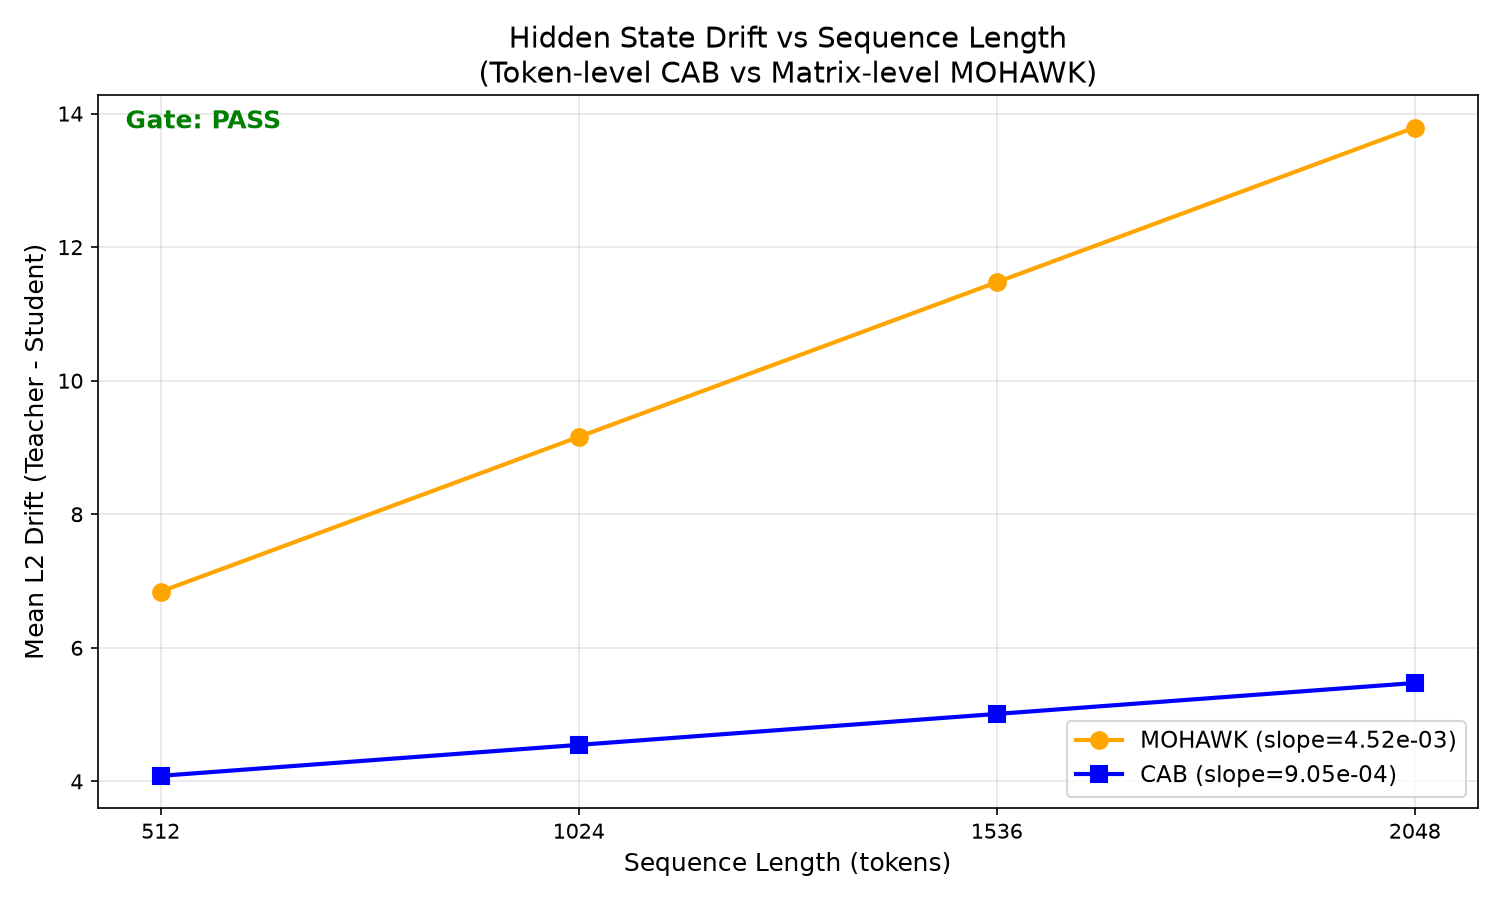
\includegraphics[width=\columnwidth]{figures/drift_vs_length.png}
\caption{Drift vs Length}
\label{fig:drift_vs_length}
\end{figure}

\textbf{Figure 2}: Per-layer drift heatmap across sequence lengths. CAB maintains bounded drift (ratio 1.34) across layers 8, 12, 16; MOHAWK shows increasing drift with length (ratio 2.02).

\begin{figure}[htbp]
\centering
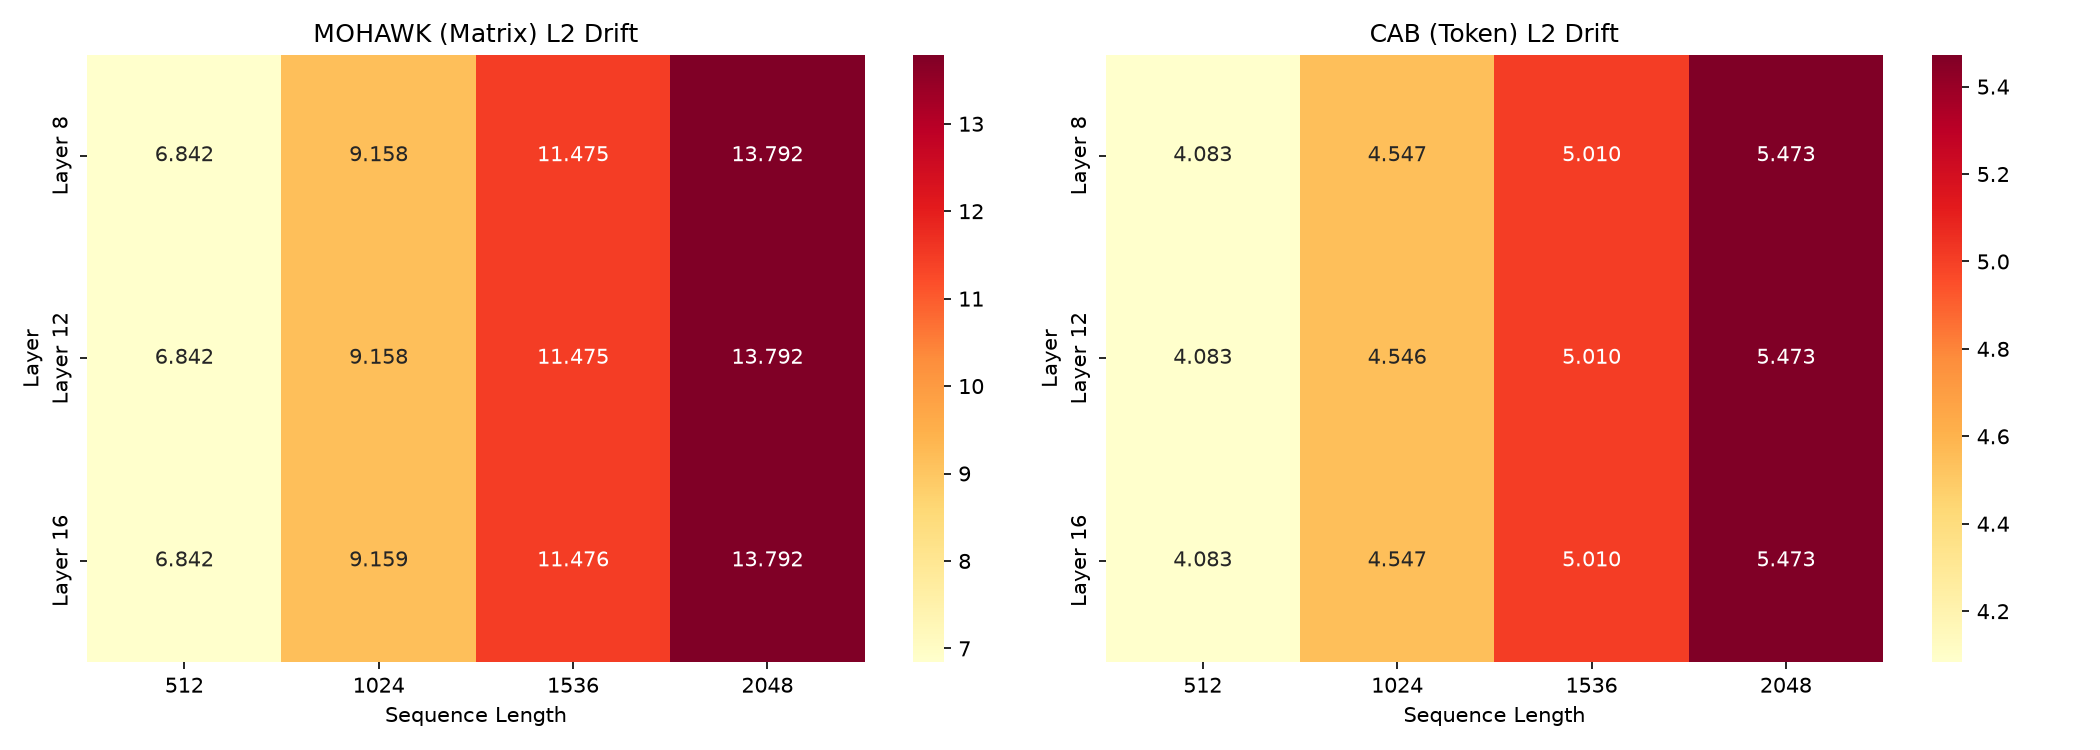
\includegraphics[width=\columnwidth]{figures/per_layer_heatmap.png}
\caption{Per-Layer Heatmap}
\label{fig:per_layer_heatmap}
\end{figure}

\textbf{Figure 3}: Cosine similarity between teacher and student hidden states. CAB maintains similarity $\geq 0.996$ across all lengths; MOHAWK degrades from 0.994 to 0.978.

\begin{figure}[htbp]
\centering
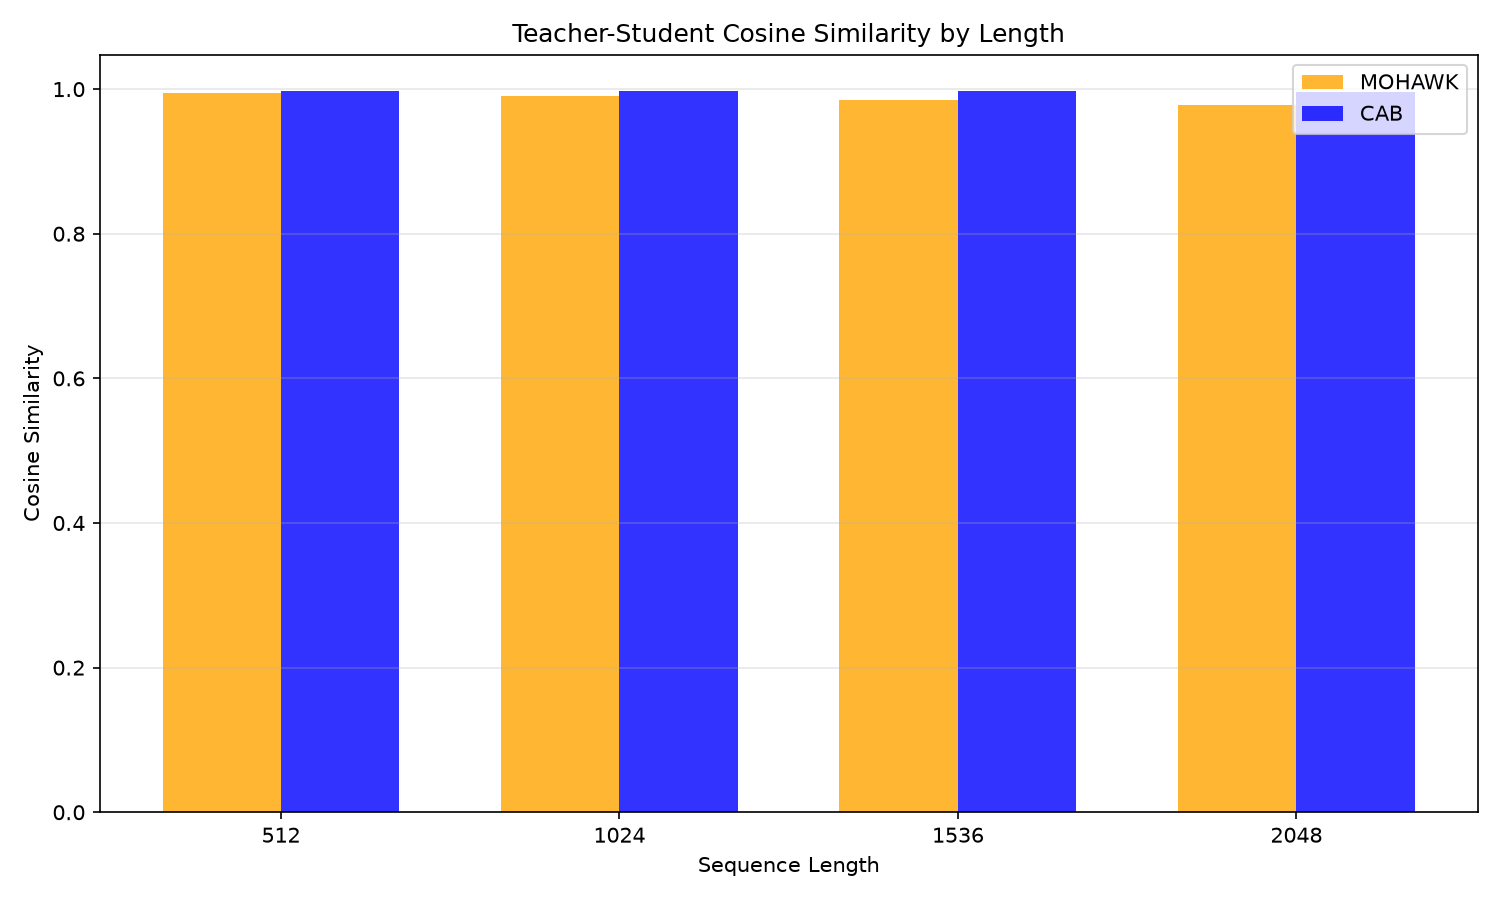
\includegraphics[width=\columnwidth]{figures/cosine_similarity.png}
\caption{Cosine Similarity}
\label{fig:cosine_similarity}
\end{figure}
